\subsubsection{Kompozitní podmínky pravidel}

Podporu kompozitních podmínek odvozovacích pravidel (vnořené aplikace logických
funkcí v podmínkách) jsem v ExiLu neimplementoval. Rád bych zde ale ukázal, proč
je implementace této funkcionality vzhledem k aktuální implementaci algoritmu
RETE složitá.

\begin{figure}[h]
\centering
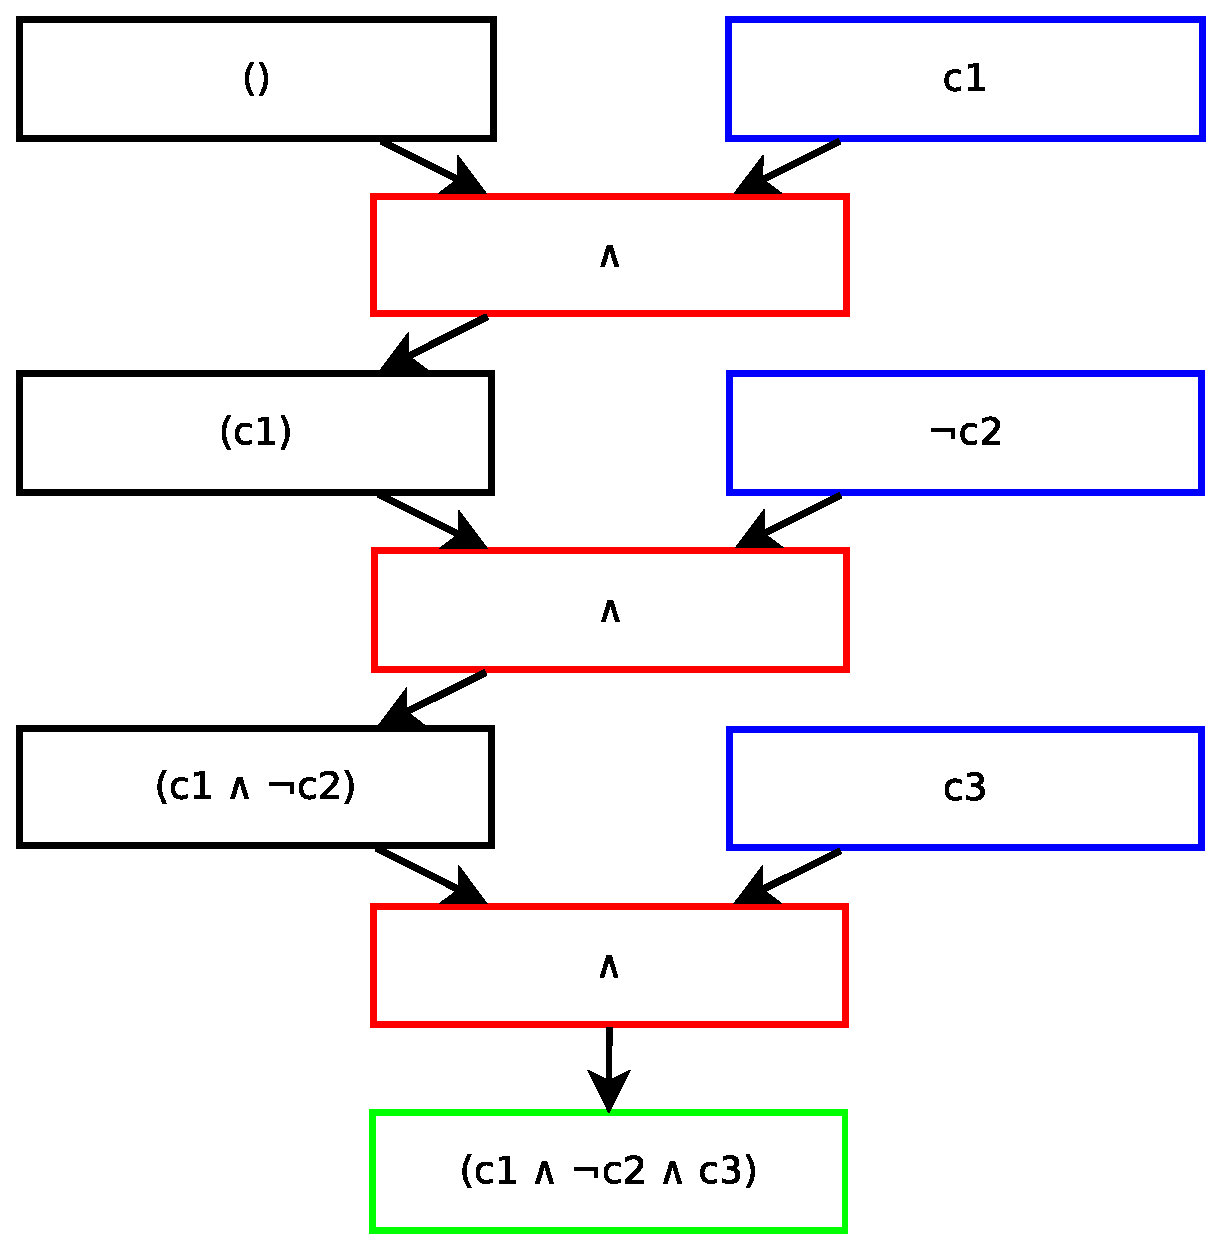
\includegraphics[height=10cm]{rete-beta-conds.eps}
\caption{Beta část sítě RETE s funkcemi uzlů}
\label{rete-beta-conds}
\end{figure}

Obrázek \ref{rete-beta-conds} ukazuje diagram beta části sítě RETE z předchozí sekce. Názvy uzlů
jsem zde ale nahradil jejich funkcí. Paměťové uzly ukládají fakty nebo tokeny
splňující jednu (v případě alpha-memory-nodů), nebo více (u beta-memory-nodů)
podmínek pravidla. Testovací (beta-join-nody) pak zajišťují agregaci těchto
faktů a tokenů. Jednu z podmínek jsem navíc pro ukázku znegoval.

Síť v diagramu splňuje několik podmínek:
\begin{enumerate}
  \item uzly jsou konstruovány ve stejném pořadí, v jakém se podmínky v definici
    pravidla vyskytují,
  \item beta-join-node vždy spojuje jeden alpha-memory-node s jedním
    beta-memory-nodem, agreguje tedy fakty splňující jednu podmínku pravidla s
    tokeny reprezentujícím posloupnost faktů splňující jeho předchozí podmínky,
  \item negace podmínky je vždy aplikována jen na úrovni jednoho faktu.
\end{enumerate}

\begin{figure}[h]
\centering
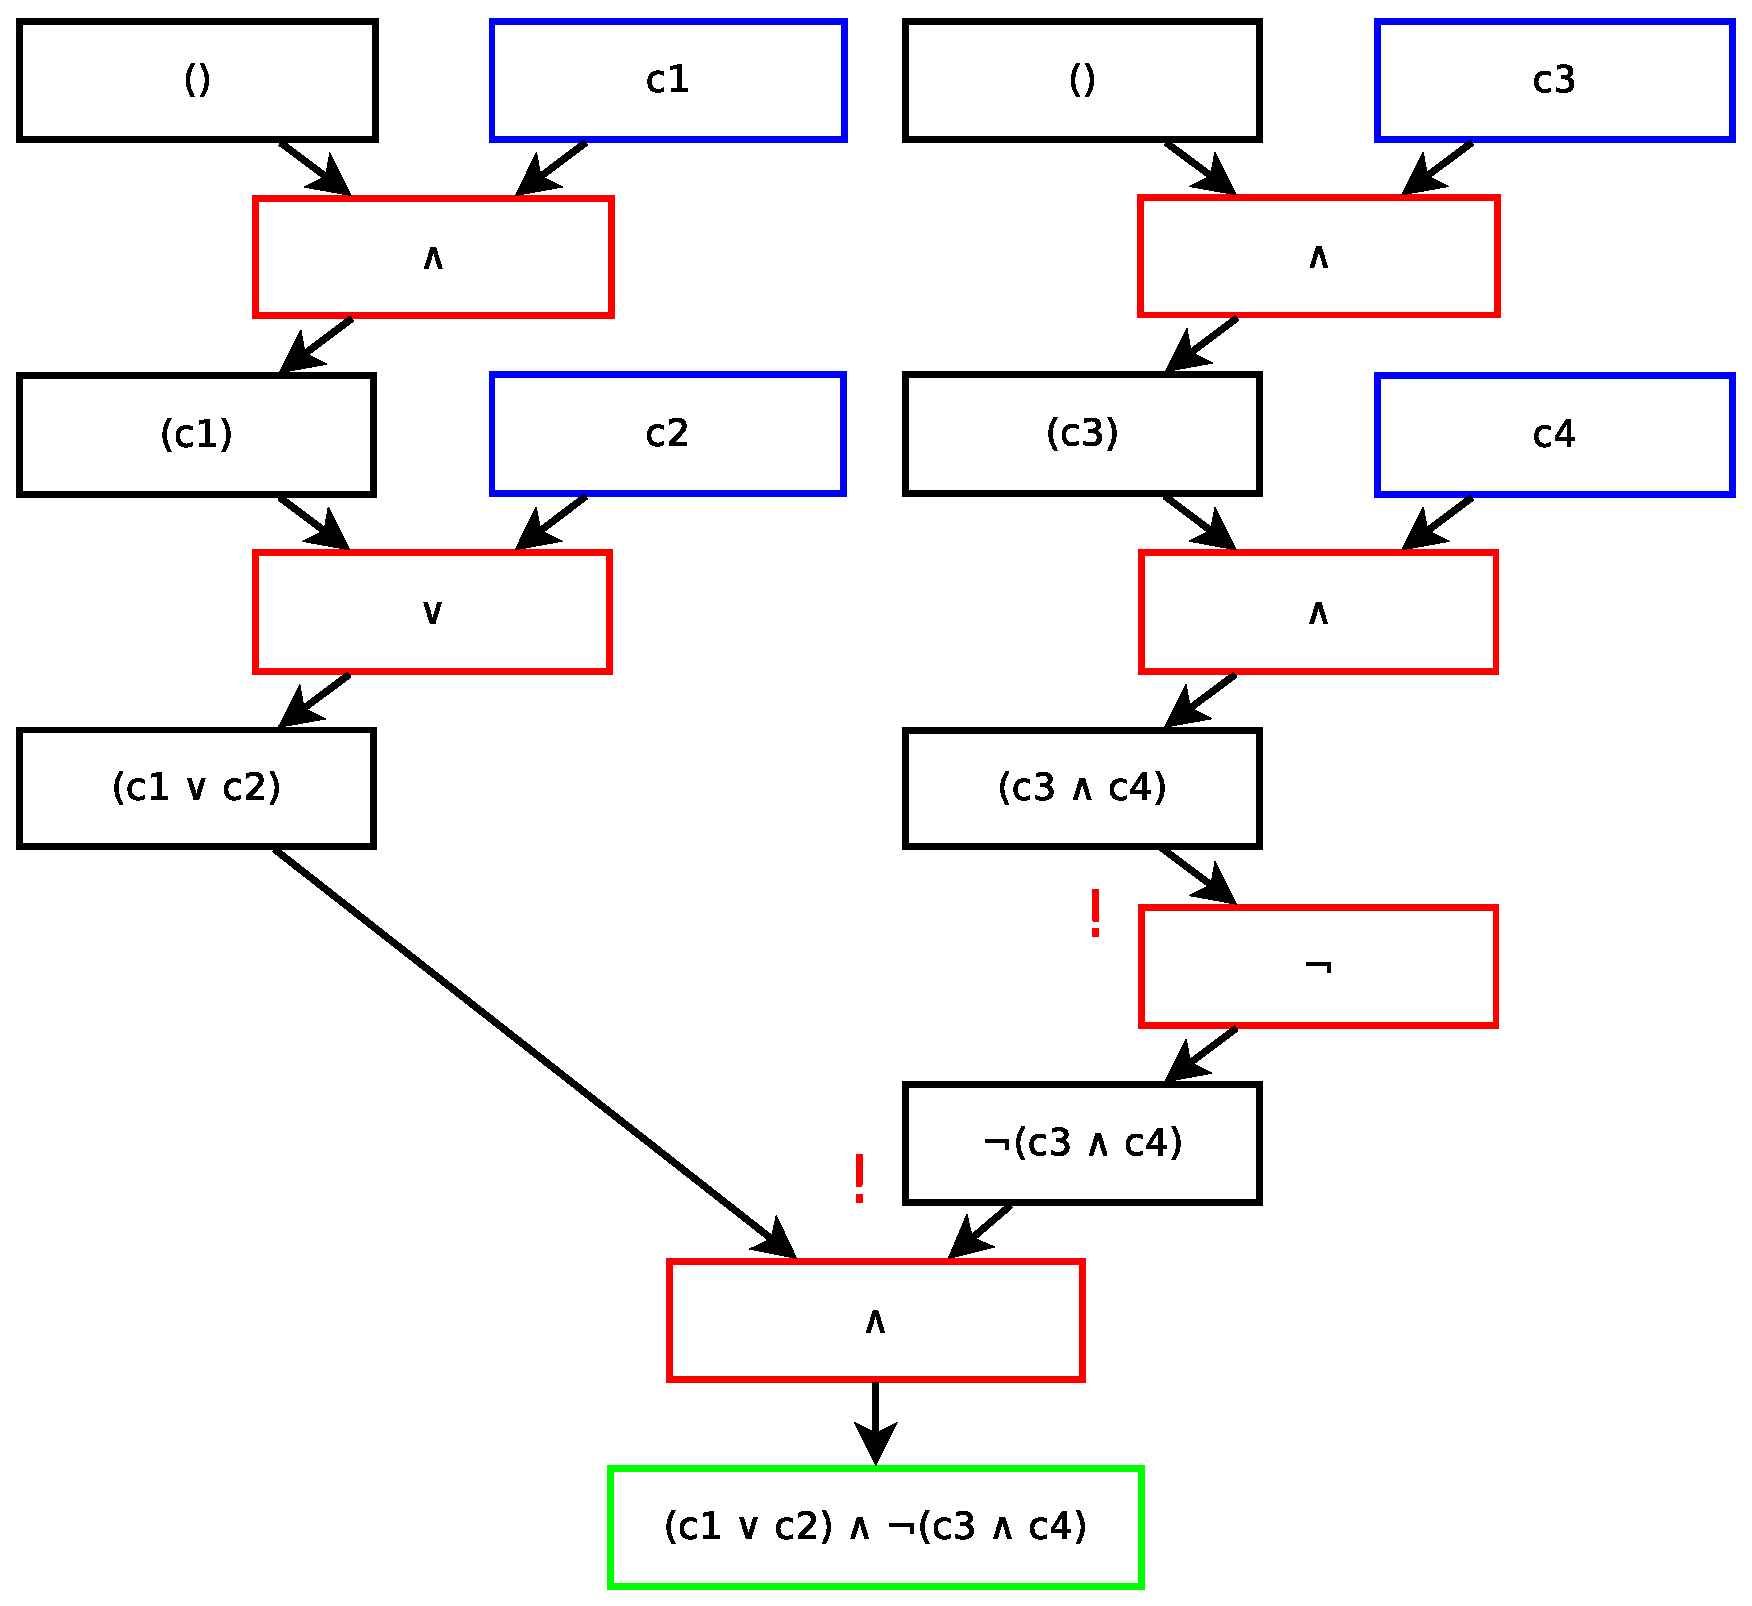
\includegraphics[height=12cm]{rete-beta-comp-conds.eps}
\caption{Beta část sítě RETE s funkcemi uzlů}
\label{rete-beta-comp-conds}
\end{figure}

Představme si nyní stavbu RETE sítě v případě následujícícho pravidla
s~kompozitními podmínkami:
\begin{minted}{cl}
(defrule rule
  (and (or condition1 condition2)
       (not (and condition3 condition4)))
  =>
  ...)
\end{minted}
Ta je zobrazena na obrázku \ref{rete-beta-comp-conds} Z diagramu vidíme, že síť porušuje všechny
uvedené podmínky.

% Z fungování beta částí sítě RETE (viz sekce \ref{rete}) vidíme, že vyhodnocování
% podmínek pravidla je inherentně sekvenční. \verb|Beta-join-nody| zde
% implementují logickou spojku \emph{a} mezi podmínkami pravidla, která je zde
% zleva asociativní.
